\documentclass[11pt]{beamer}
\usetheme{Berlin}
\usepackage[utf8]{inputenc}
\usepackage[english]{babel}
\usepackage{amsmath}
\usepackage{amsfonts}
\usepackage{amssymb}
\usepackage{graphicx}
\usepackage{xcolor}
\usepackage{booktabs}
\usepackage{pgfpages}
\usepackage{tikz}
\usetikzlibrary{shapes,arrows,positioning,calc}
\author{Adam Aili \& Erik Ekelund}
\title{Model-Based Development of an Underwater Vehicle}
%\setbeamercovered{transparent} 
\setbeamertemplate{navigation symbols}{} 
%\logo{} 
%\institute{} 
\date{June 10} 
%\subject{} 
\setbeamertemplate{caption}{\insertcaption}
%\setbeameroption{show notes}
\setbeameroption{show notes on second screen=right}

\begin{notation}% Passing the option "old" to the notation environment will redefine the notationtabular environment so that it produces an old style LaTeX tabular instead of a ctable.sty style tabular.
  \centering
  
% Lägg in förkortningarna i bokstavsordning!
  \begin{notationtabular}{Abbreviations}{Abbreviation}{Description}
    \abbrCB\index{CB@\abbrCG!abbreviation} & Center of buoyancy. \\
    \abbrCG\index{CG@\abbrCG!abbreviation} & Center of gravity. \\
    \abbrCO\index{CO@\abbrCO!abbreviation} & Center of origin. \\
    \abbrDOF\index{DOF@\abbrDOF!abbreviation} & Degrees of freedom. \\
    \abbrEKF\index{EKF@\abbrEKF!abbreviation} & Extended Kalman filter.\\
    \abbrESC\index{ESC@\abbrESC!abbreviation} & Electronic speed controller.\\
    \abbrIMU\index{IMU@\abbrIMU!abbreviation} & Inertial measurement unit.\\
    \abbrIO\index{I/O@\abbrIO!abbreviation}   & Input/Output.\\
    \abbrKF\index{KF@\abbrKF!abbreviation}	& Kalman filter.\\
    \abbrMPC\index{MPC@\abbrMPC!abbreviation} & Model predictive control.\\
    \abbrPID\index{PID@\abbrPID!abbreviation} & Proportional, integral, differential (regulator). \\
    \abbrPI\index{PI@\abbrPI!abbreviation} & Proportional, integral (regulator). \\
    \abbrRPM\index{RPM@\abbrRPM!abbreviation} & Rotations per minute. \\
    \abbrSLAM\index{SLAM@\abbrSLAM!abbreviation} & Simultaneous localisation and mapping. \\
    \abbrSNR\index{SNR@\abbrSNR!abbreviation} & Signal to noise ratio. \\
    \abbrROS\index{ROS@\abbrROS!abbreviation} & Robot Operating System. \\
    \abbrROV\index{ROV@\abbrROV!abbreviation} & Remotely operated vehicle. \\
    \abbrUV\index{UV@\abbrUV!abbreviation} & Unmanned vehicle. \\

    
    
  \end{notationtabular}
  
\end{notation}


\begin{document}


\begin{frame}
\titlepage
\end{frame}
%%%%%%%%%%%%%%%%%%%%%Intro%%%%%%%%%%%%%%%%%%%%%%%%%%%%%%%%%%%%%%%%%%%%%%%%%%%%%%%%%%%%%%%%%%%%%%%%%
\begin{frame}
\begin{itemize}
\item Model-based design development
\item Control system
\end{itemize}
\note{Purpose of model-based design development}
\note{Purpose of a control system}
\end{frame}

\begin{frame}
\begin{itemize}
\item Assemble the ROV.
\item Develop a framework for changing controller in the ROV.
\item Estimate a model of the ROV.
\item Create a plant model of the ROV in Matlab/Simulink.
\item Develop a robust model-based controller and evaluate its performance with simulations and tests.
\end{itemize}
\end{frame}


%%%%%%%%%%%%%%%%%%%%%Rov platfrom%%%%%%%%%%%%%%%%%%%%%%%%%%%%%%%%%%%%%%%%%%%%%%%%%%%%%%%%%%%%%%%%%%
\section{ROV Platform}
\begin{frame}
Bluerov
I/O
sensorfusion
\end{frame}
%%%%%%%%%%%%%%%%%%%%%Model%%%%%%%%%%%%%%%%%%%%%%%%%%%%%%%%%%%%%%%%%%%%%%%%%%%%%%%%%%%%%%%%%%
\section{Modelling the ROV}
\begin{frame}
what is a model and be used for
damping - linear quadratic
Coriolis
restoring forces
added mass and added moment of inertia
simplifications and why they are needed
\end{frame}
%%%%%%%%%%%%%%%%%%%%%Parameter Estimation%%%%%%%%%%%%%%%%%%%%%%%%%%%%%%%%%%%%%%%%%%%%%%%%%%%%%%%%%%%%%%%%%%
\section{Parameter Estimation}
\begin{frame}
What is parameter estimation and why is it needed
pem and problems
kalman smoother
pem results
kalman estimation
kalman results
discussion
\end{frame}

%%%%%%%%%%%%%%%%%%%%%Controllers%%%%%%%%%%%%%%%%%%%%%%%%%%%%%%%%%%%%%%%%%%%%%%%%%%%%%%%%%%%%%%%%%%

\section{Controllers}
\begin{frame}
\begin{itemize}
\item<1->  Automatic control - What is it?
\item<2->  Open-loop control
\item<3->  Feed-back control
\item<4->  Exact linearisation
\end{itemize}
\only<2-2>{
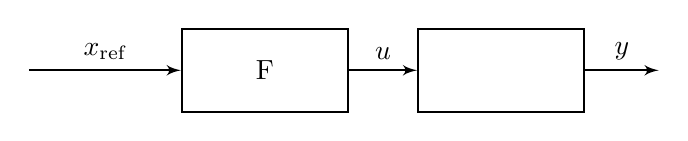
\begin{tikzpicture}[auto, thick, node distance=2cm,>=latex',
 block/.style  = {draw, rectangle,minimum height=3em, minimum width=6em},
 sum/.style    = {draw, circle, inner sep=0pt, text width=4mm,align=center, node distance=1cm},
 input/.style  = {coordinate},
 output/.style = {coordinate},
 pinstyle/.style = {pin edge={to-,thin,black}}]
 
 \node [input, name=input] {};
 \node [block, right of=input, node distance=3cm] (controller) {F};
 \node [block, right of=controller, node distance=3cm] (system) {\abbrROV};

 \draw [->] (controller) -- node[name=u] {$u$} (system);
 \node [output, right of=system] (output) {};

 \draw [draw,->] (input) -- node {$x_{\text{ref}}$} (controller);
 \draw [->] (system) -- node [name=y] {$y$}(output);
\end{tikzpicture}
}
\only<3-3>{
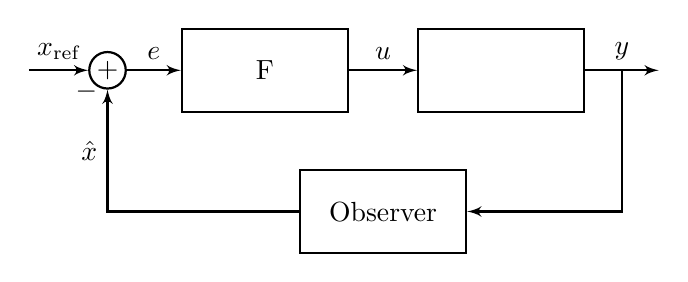
\begin{tikzpicture}[auto, thick, node distance=2cm,>=latex',
			 block/.style  = {draw, rectangle,minimum height=3em, minimum width=6em},
			 sum/.style    = {draw, circle, inner sep=0pt, text width=4mm,align=center, node distance=1cm},
			 input/.style  = {coordinate},
			 output/.style = {coordinate},
			 pinstyle/.style = {pin edge={to-,thin,black}}]
			 
		    \node [input, name=input] {};
		    \node [sum, right of=input] (sum) {+};
		    \node [block, right of=sum] (controller) {F};
		    \node [block, right of=controller, node distance=3cm] (system) {\abbrROV};
		
		    \draw [->] (controller) -- node[name=u] {$u$} (system);
		    \node [output, right of=system] (output) {};
		    \node [block, below of=u] (sensorfusion) {Observer};
		
		    \draw [draw,->] (input) -- node {$x_{\text{ref}}$} (sum);
		    \draw [->] (sum) -- node {$e$} (controller);
		    \draw [->] (system) -- node [name=y] {$y$}(output);
		    \draw [->] (y) |- (sensorfusion);
		    \draw [->] (sensorfusion) -| node[pos=0.99] {$-$} 
		        node [near end] {$\hat{x}$} (sum);
		\end{tikzpicture}
}
\only<4-4>{\begin{center}Consider the non-linear system\\
$\begin{bmatrix}
\dot{x}_1\\
\dot{x}_2
\end{bmatrix}=
\begin{bmatrix}
x_2\\
-a x_1 - b x_2\abs{x_2} + u
\end{bmatrix}$
\end{center}
}
\only<5-5>{\begin{center}Choose the following control strategy\\
$u = a x_1 +b x_2\abs{x_2} + \bar{u}$
\end{center}
}
\only<6-6>{\begin{center}This will give the linear system\\
$\begin{bmatrix}
\dot{x}_1\\
\dot{x}_2
\end{bmatrix}=
\begin{bmatrix}
x_2\\
\bar{u}
\end{bmatrix}$
\end{center}
}
\note{To control a system towards a desired state using input}
\note{To control the system without measuring the current state. Needs to be modelled in order to attain good performance.}
\note{To base the control action on measurements from outputs of the system.}
\note{To compensate for a systems non-linearities using a model of the system.}

%what is automatic control
%open-loop control
%exact linearisation
%attitude 
%angular velocity
%depth 
%results
%discussion
\end{frame}
\begin{frame}
\begin{center}
Attitude controller using exact linearisation.
\end{center}
\note{An attitude controller has been developed using the exact linearisation technique described earlier.}
\end{frame}
\begin{frame}
\only<1-1>{
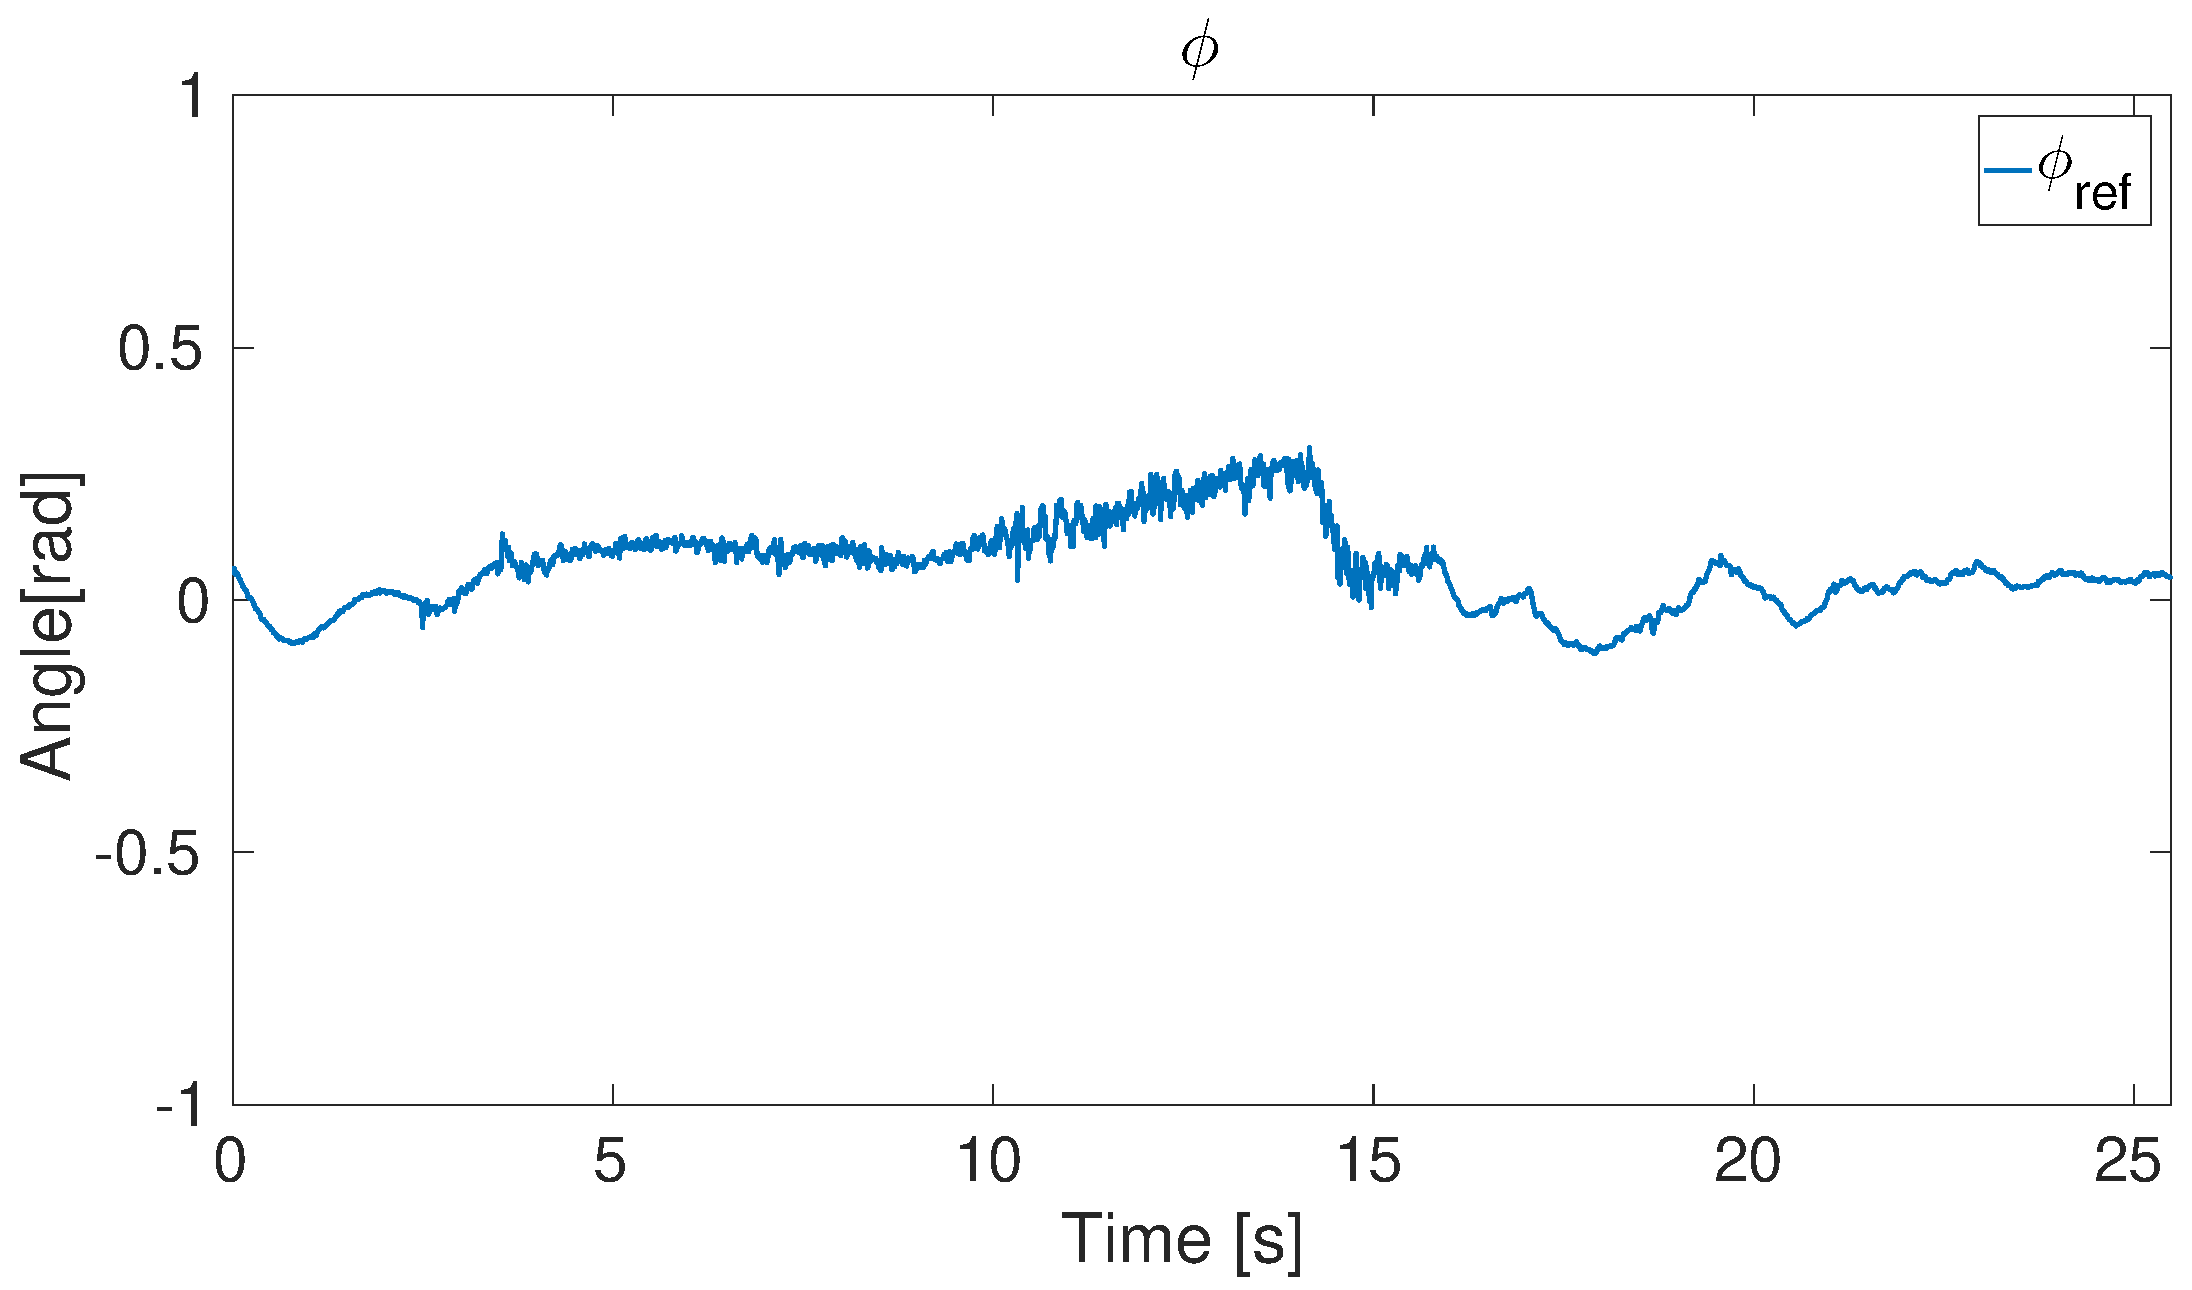
\includegraphics[scale=0.28]{../Master/fig/testExactLinAttitudePhi}
}
\only<2-2>{
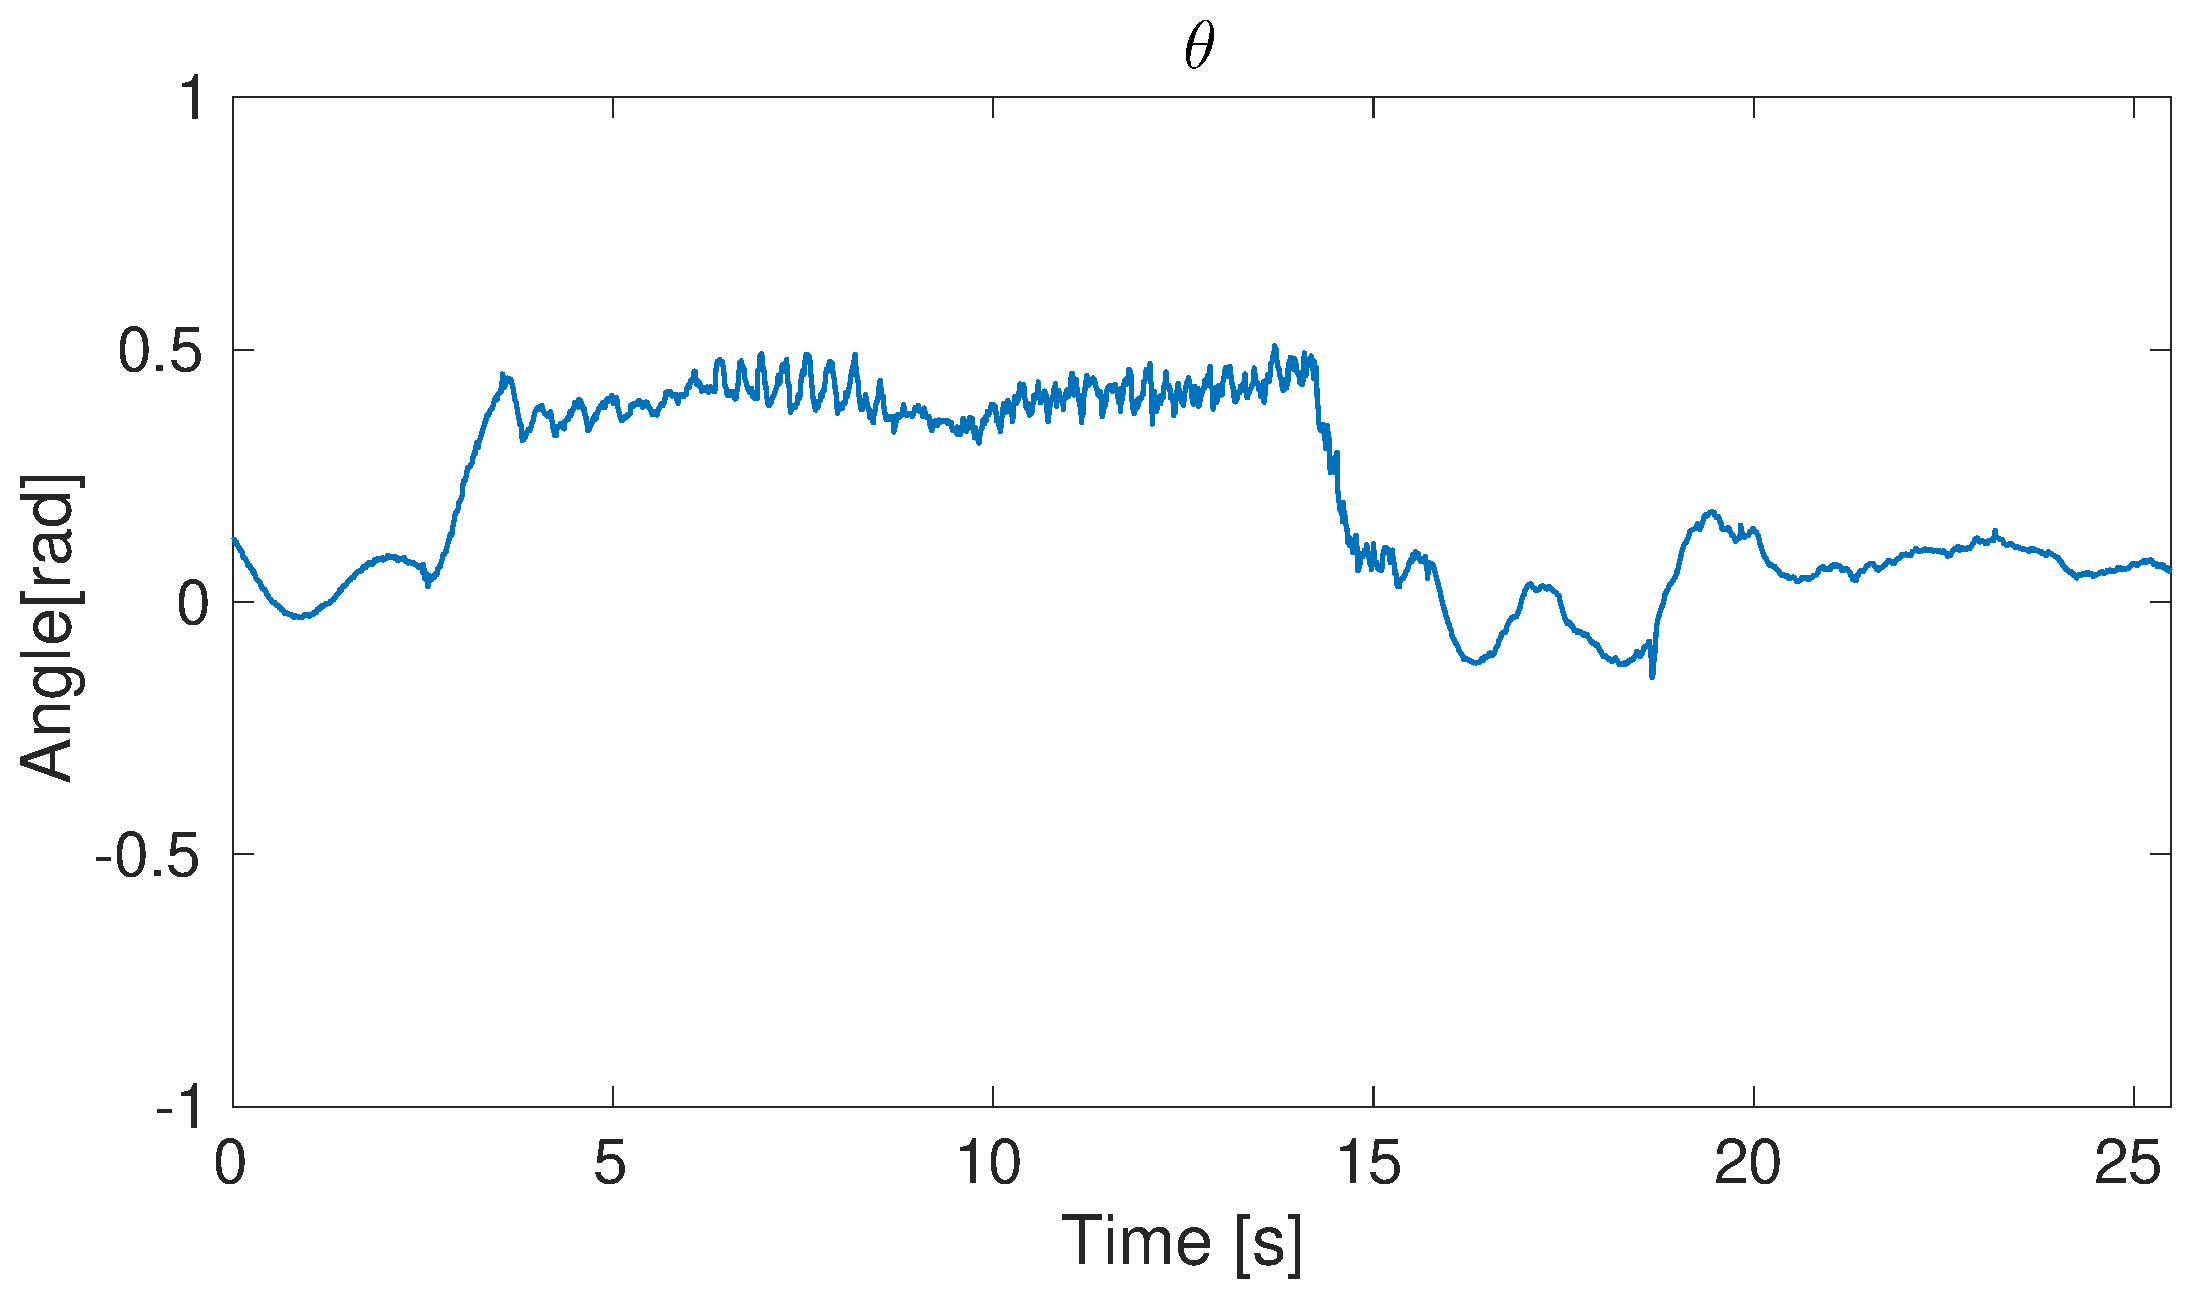
\includegraphics[scale=0.28]{../Master/fig/testExactLinAttitudeTheta}
}
\only<3-3>{
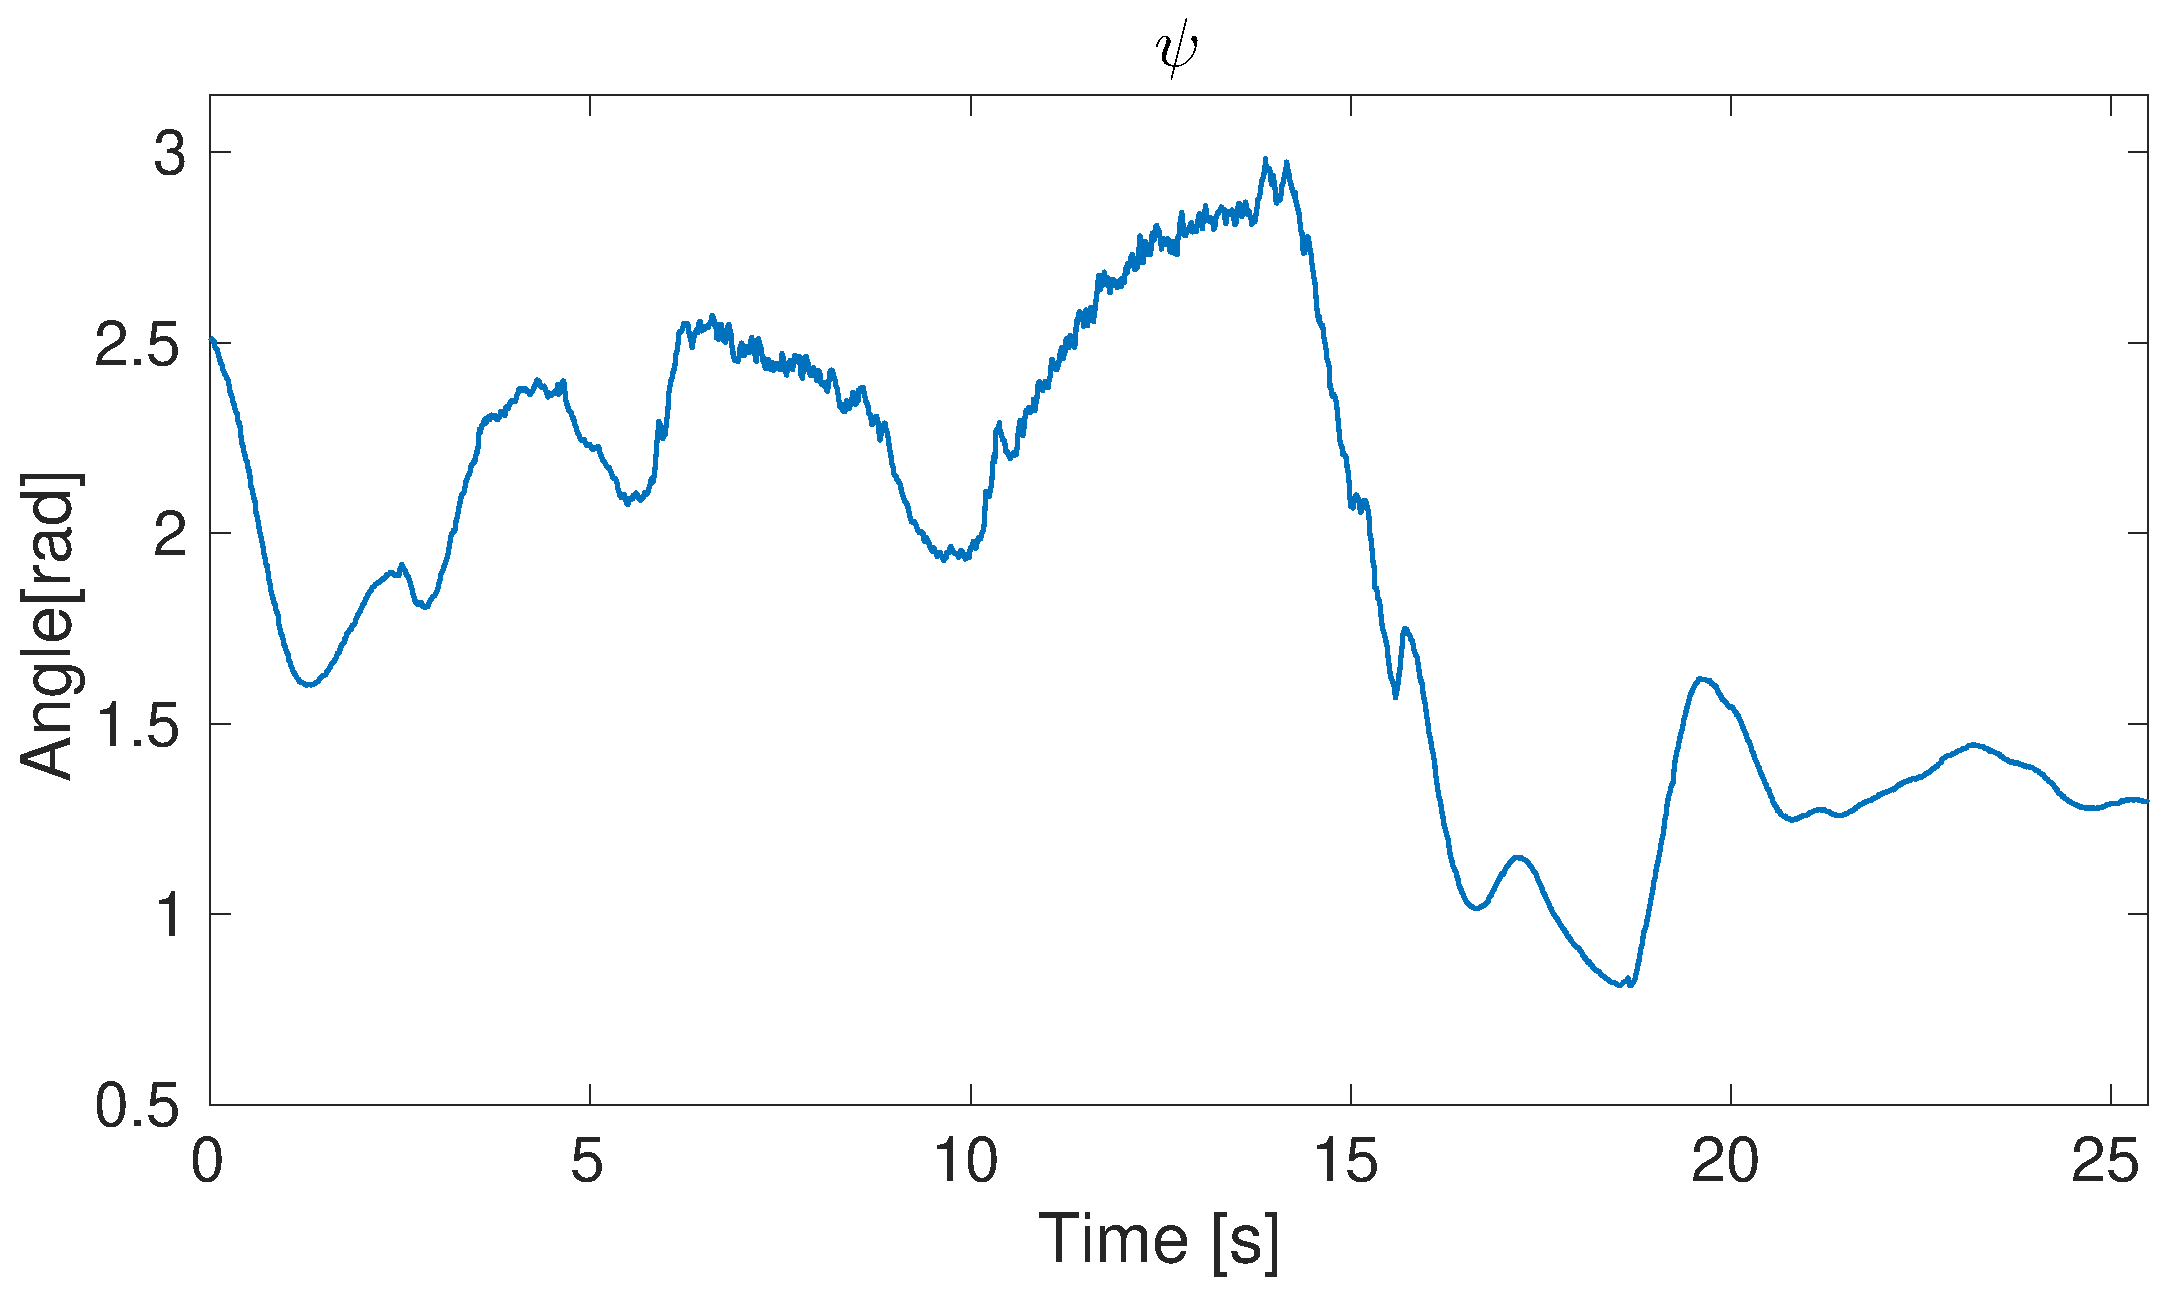
\includegraphics[scale=0.28]{../Master/fig/testExactLinAttitudePsi}
}
\end{frame}
\begin{frame}

\begin{center}
Attitude controller \textbf{without} exact linearisation.
\end{center}
\note{An attitude controller has been developed using the exact linearisation technique described earlier.}
\end{frame}


\begin{frame}
\only<1-1>{
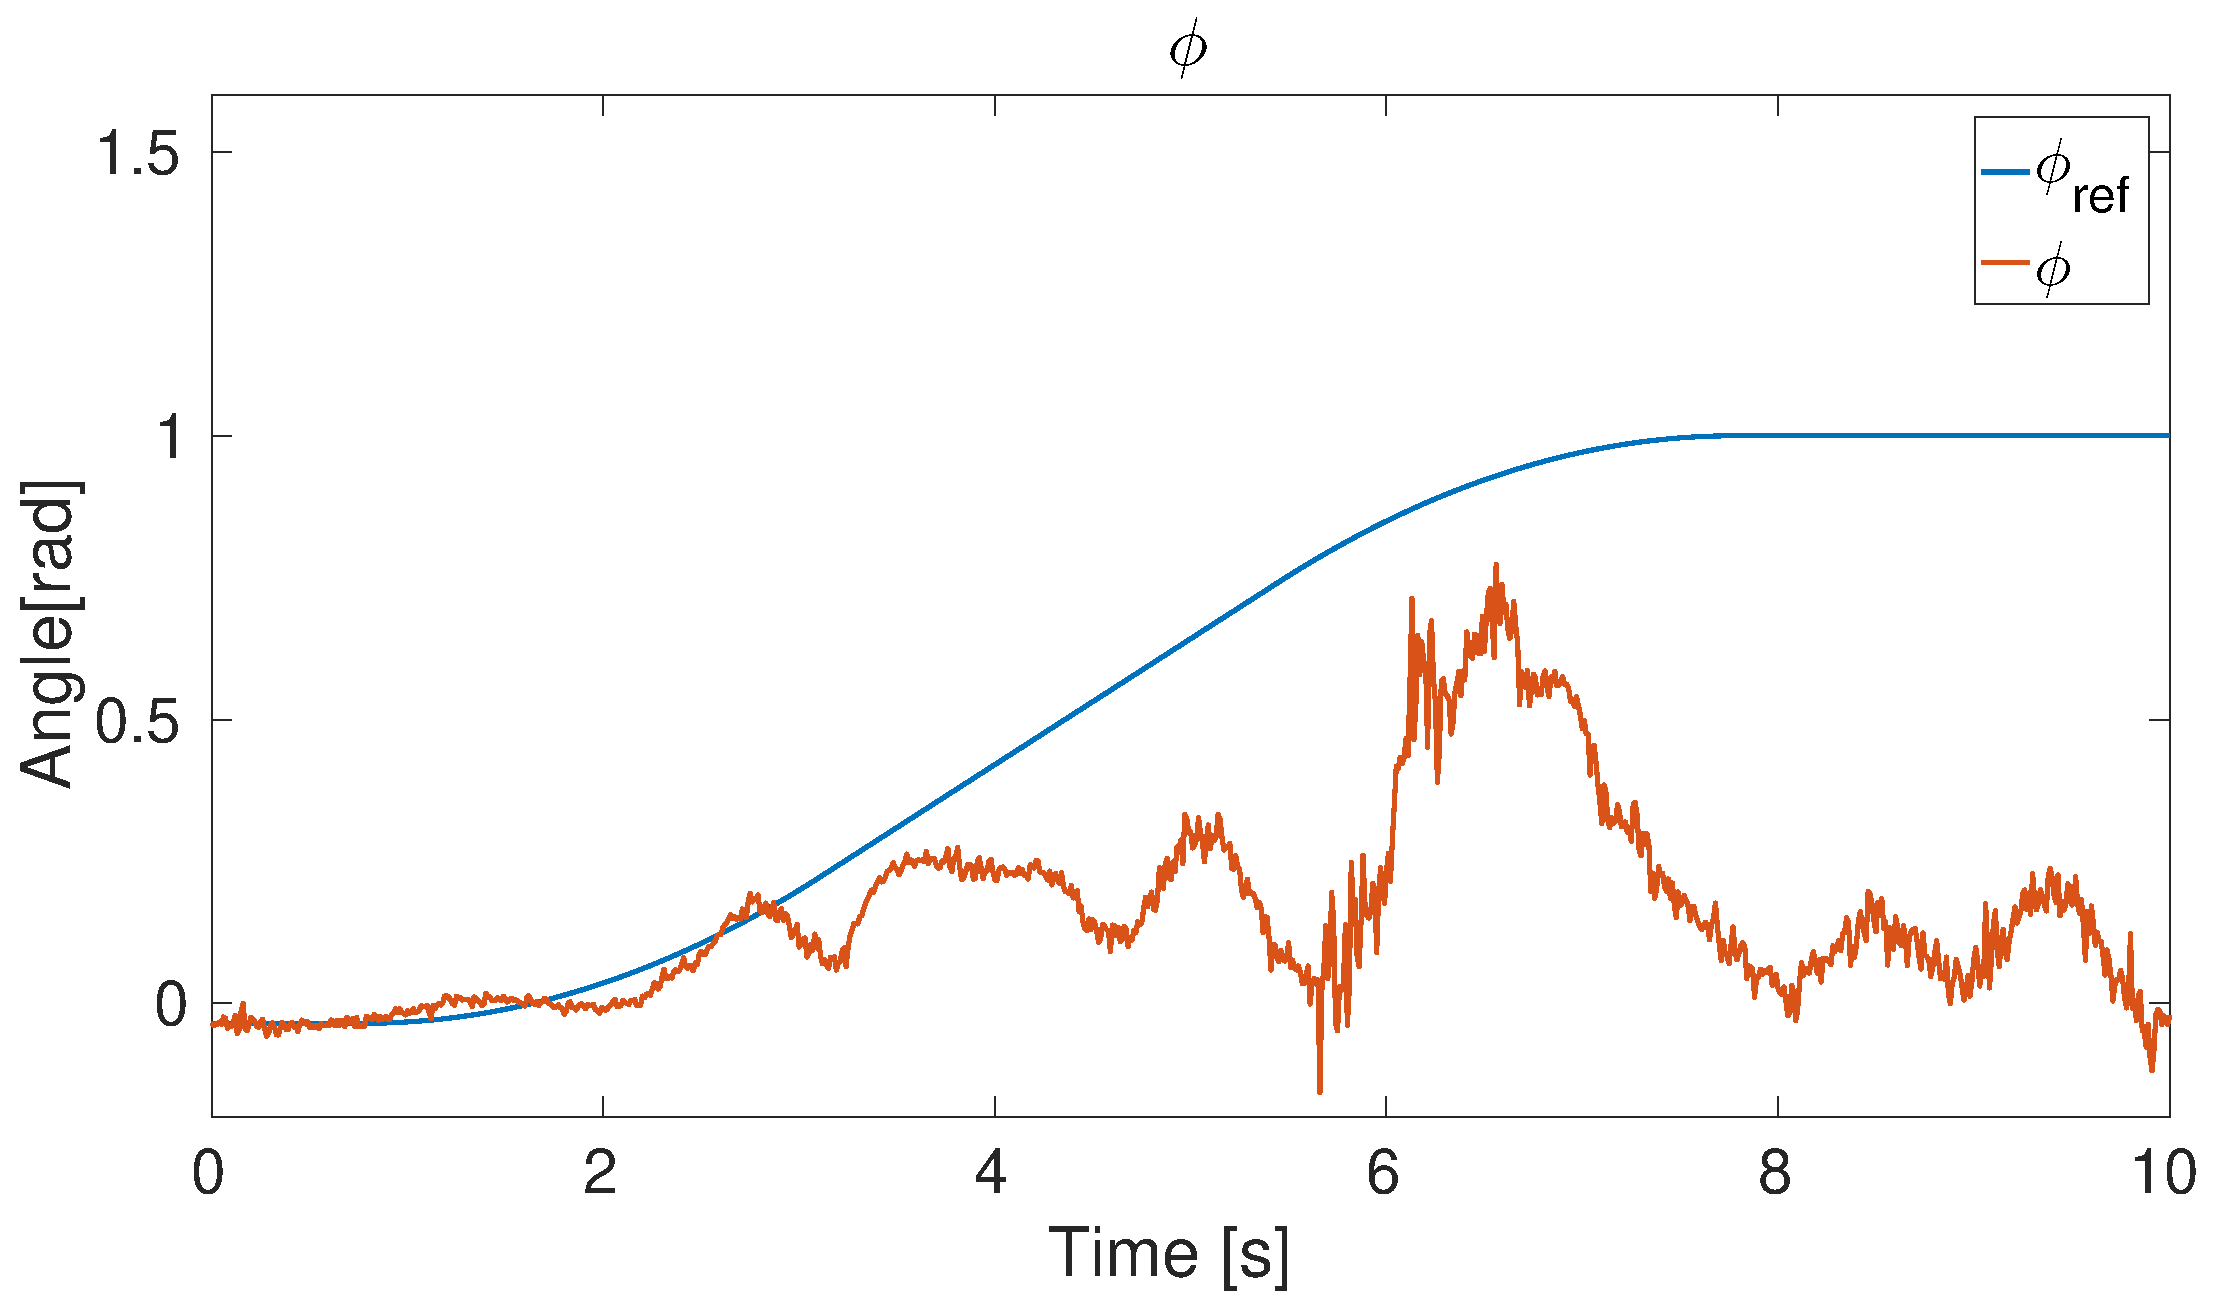
\includegraphics[scale=0.28]{../Master/fig/testStepAllPhis3e10a1}
}
\only<2-2>{
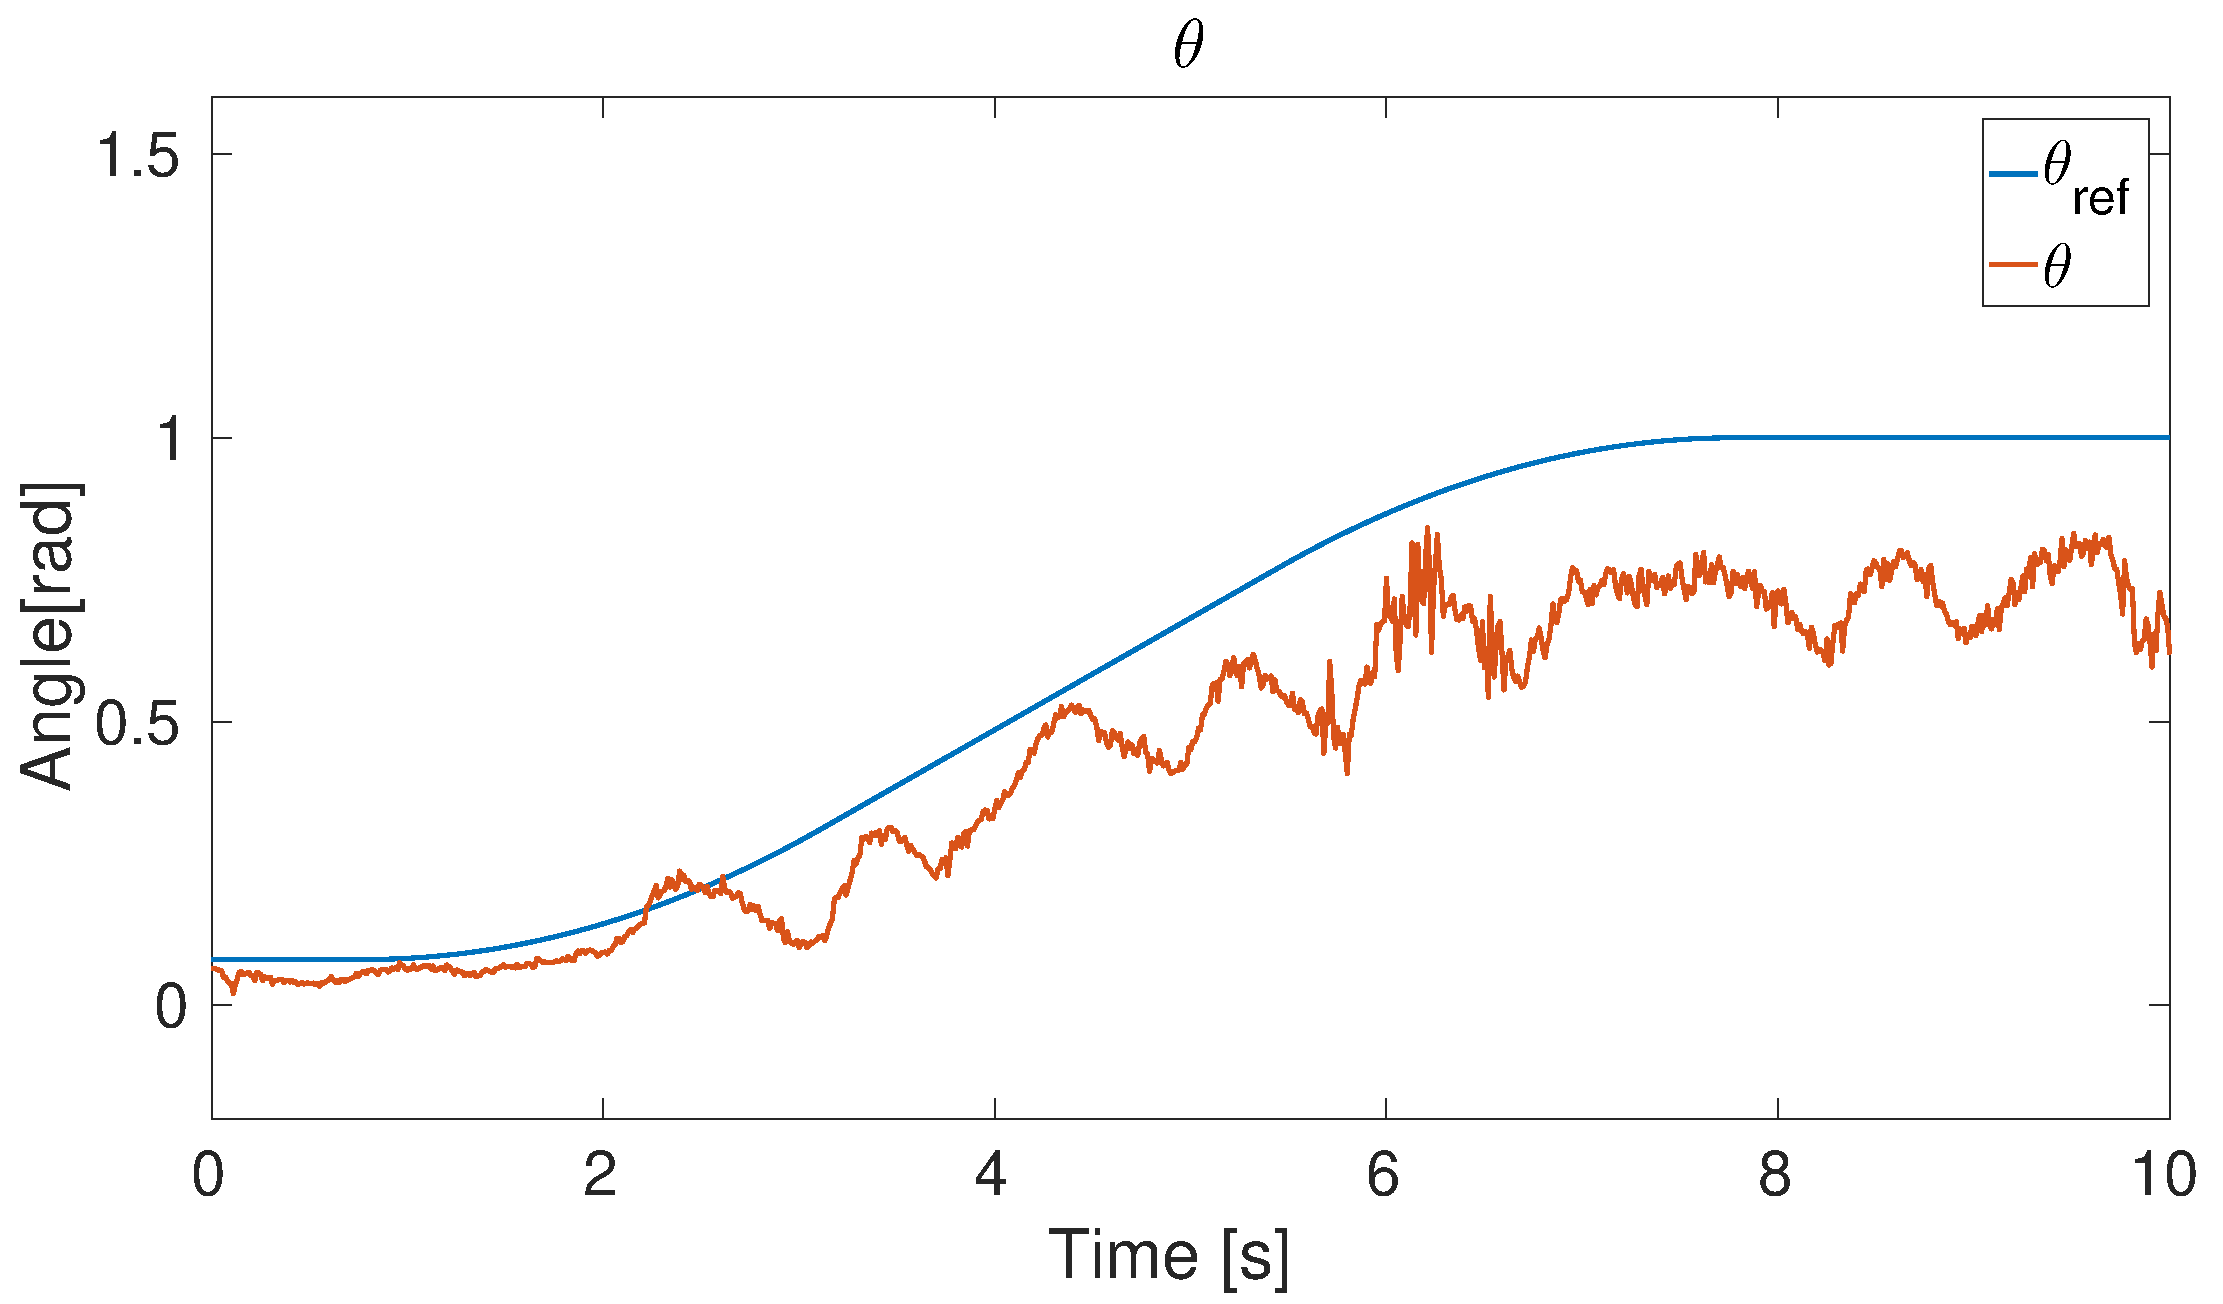
\includegraphics[scale=0.28]{../Master/fig/testStepAllThetas3e10a1}
}
\only<3-3>{
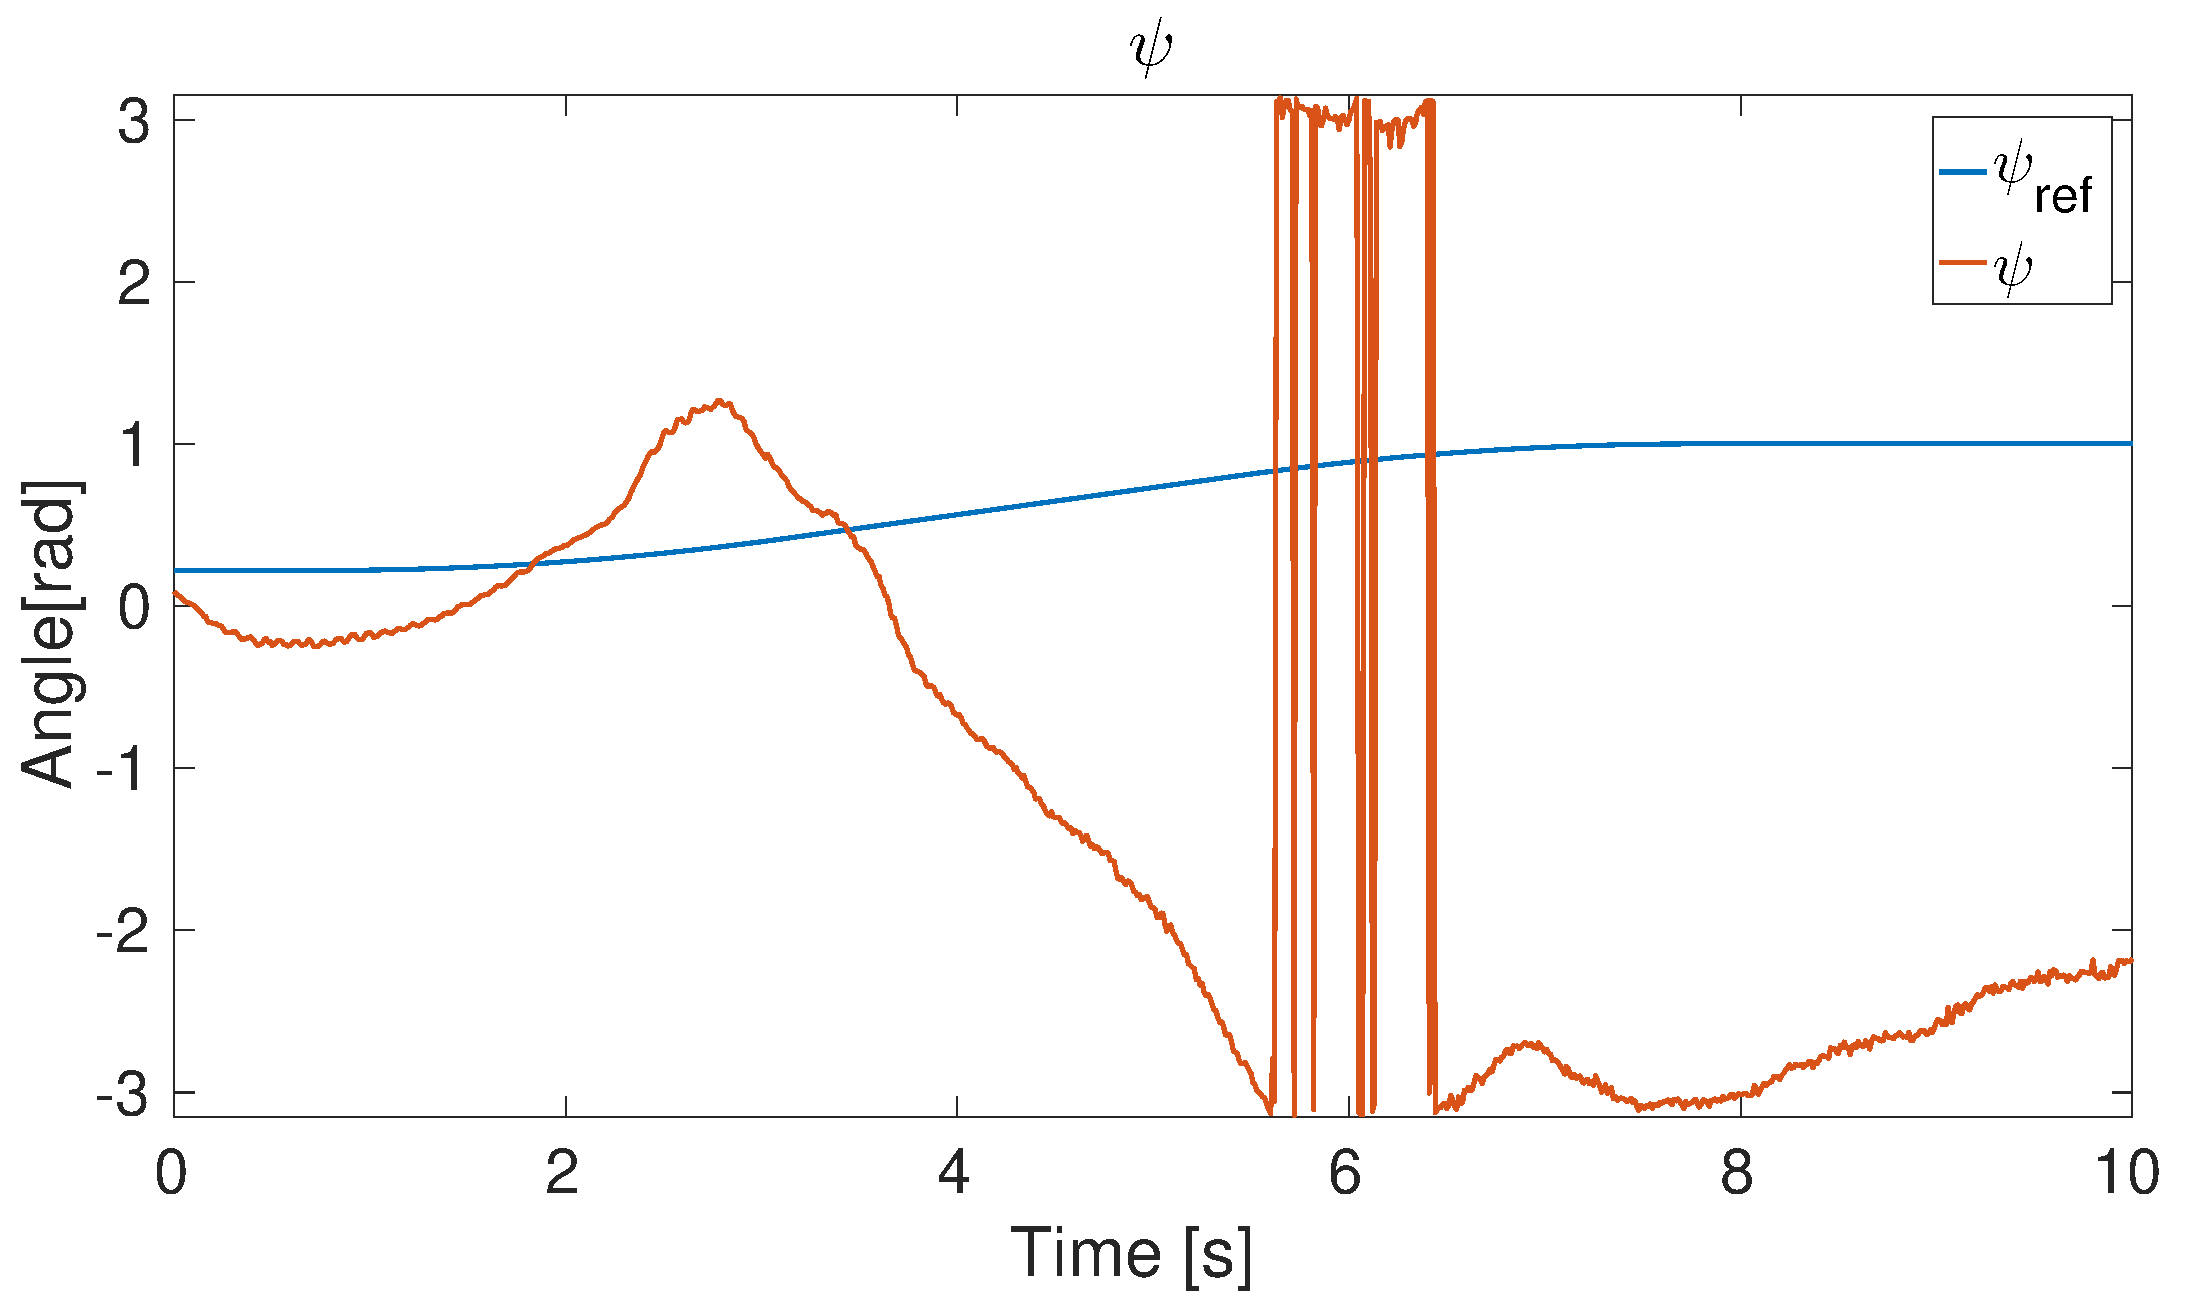
\includegraphics[scale=0.28]{../Master/fig/testStepAllPsis3e10a1}
}
\end{frame}

\begin{frame}
\only<1-1>{
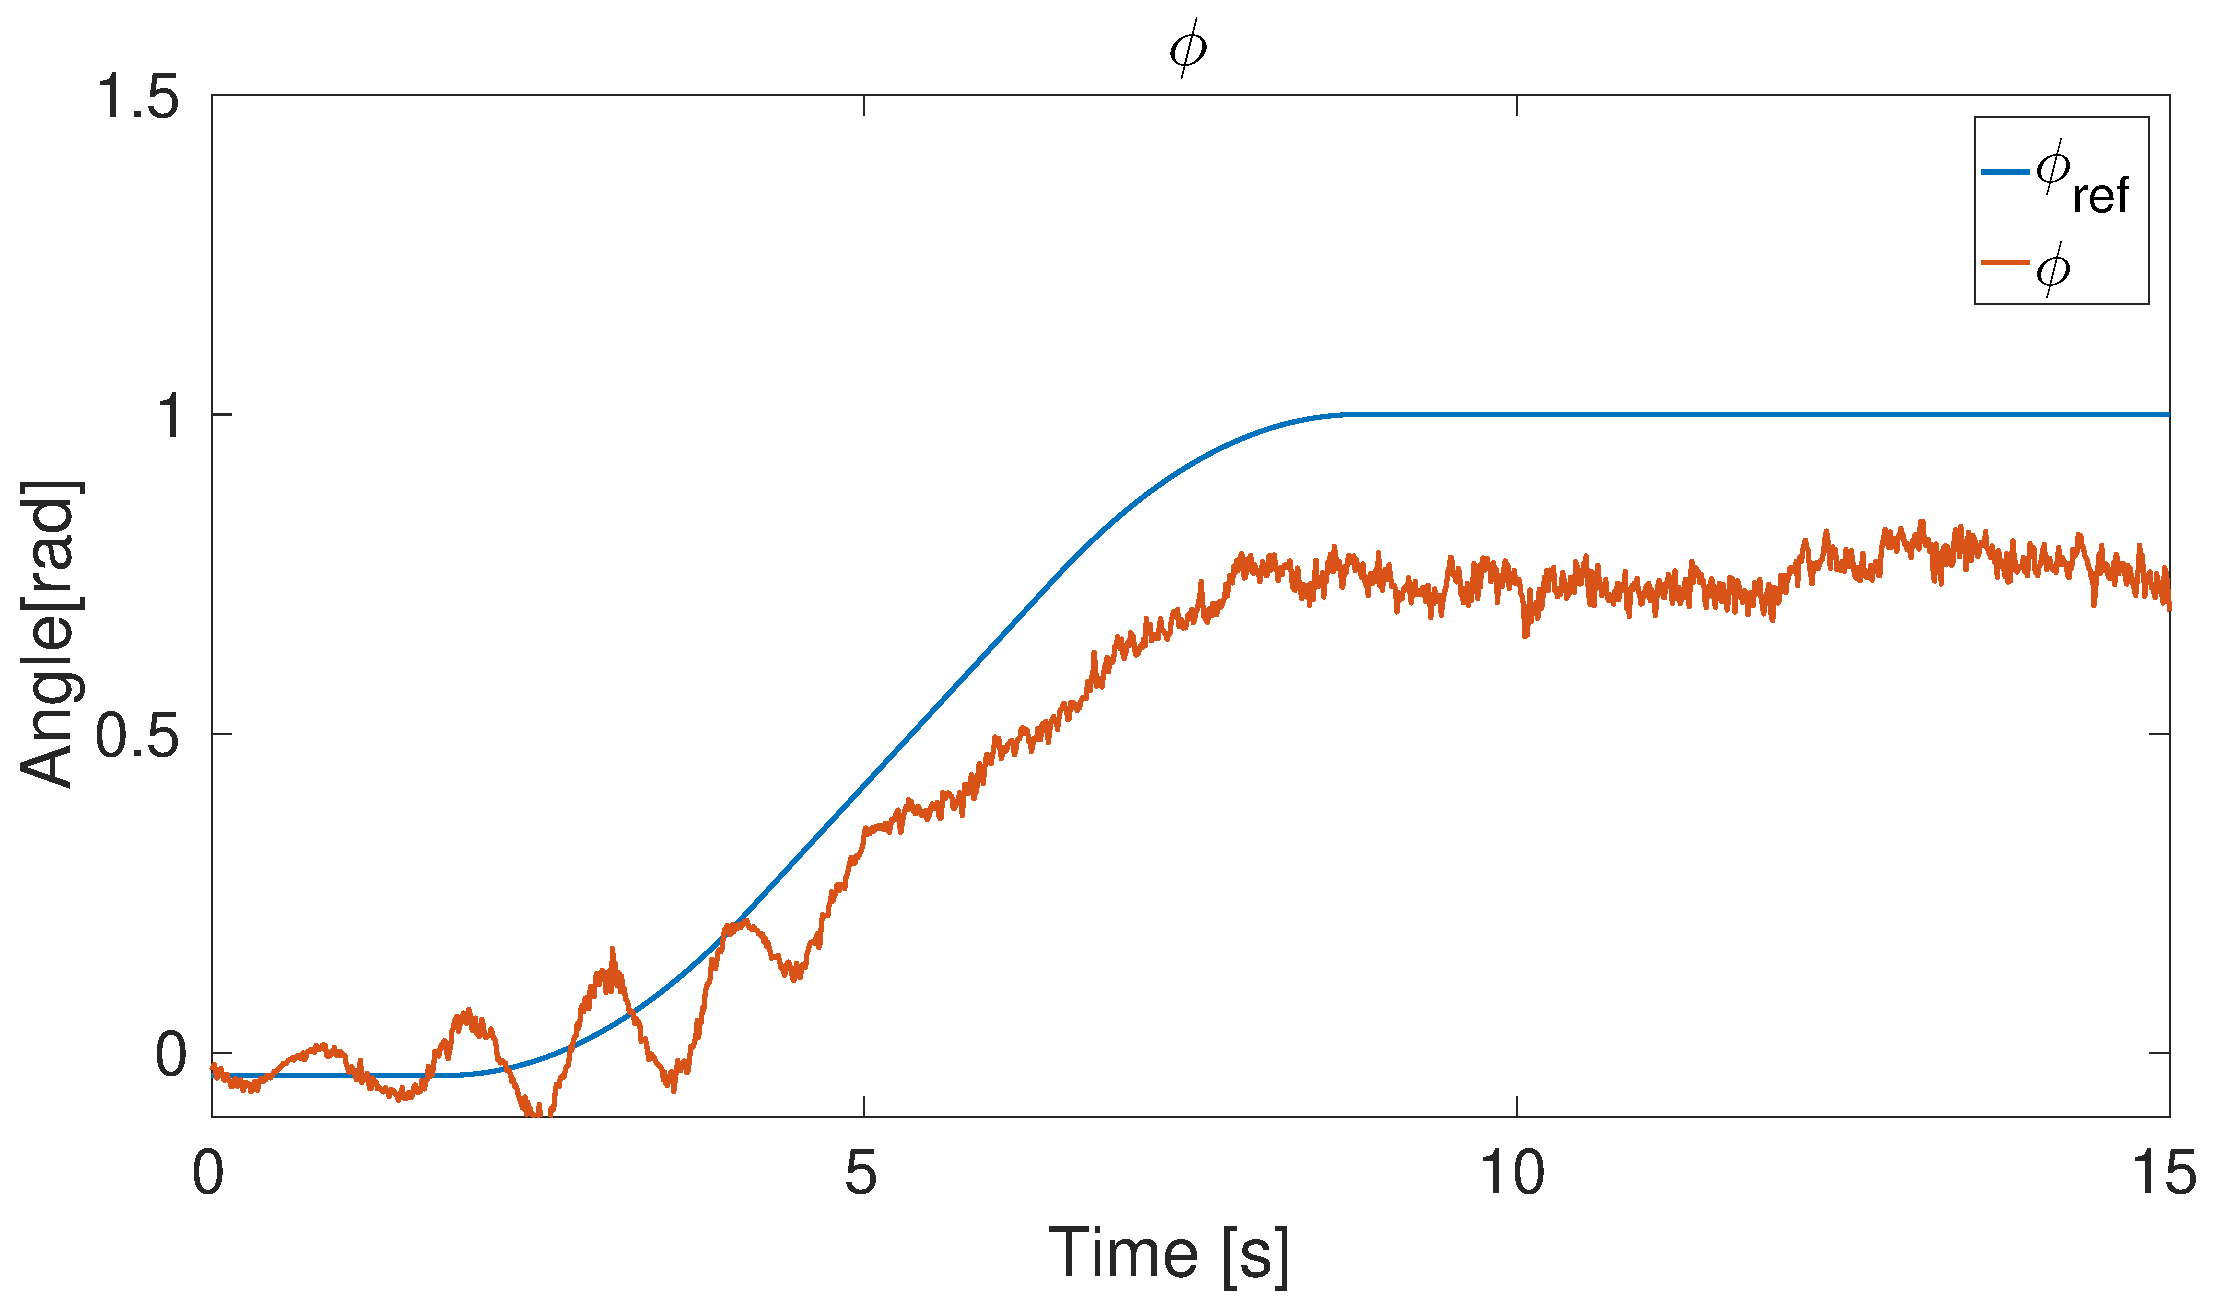
\includegraphics[scale=0.28]{../Master/fig/testStepThetaPhiPhis3e10a1}
}
\only<2-2>{
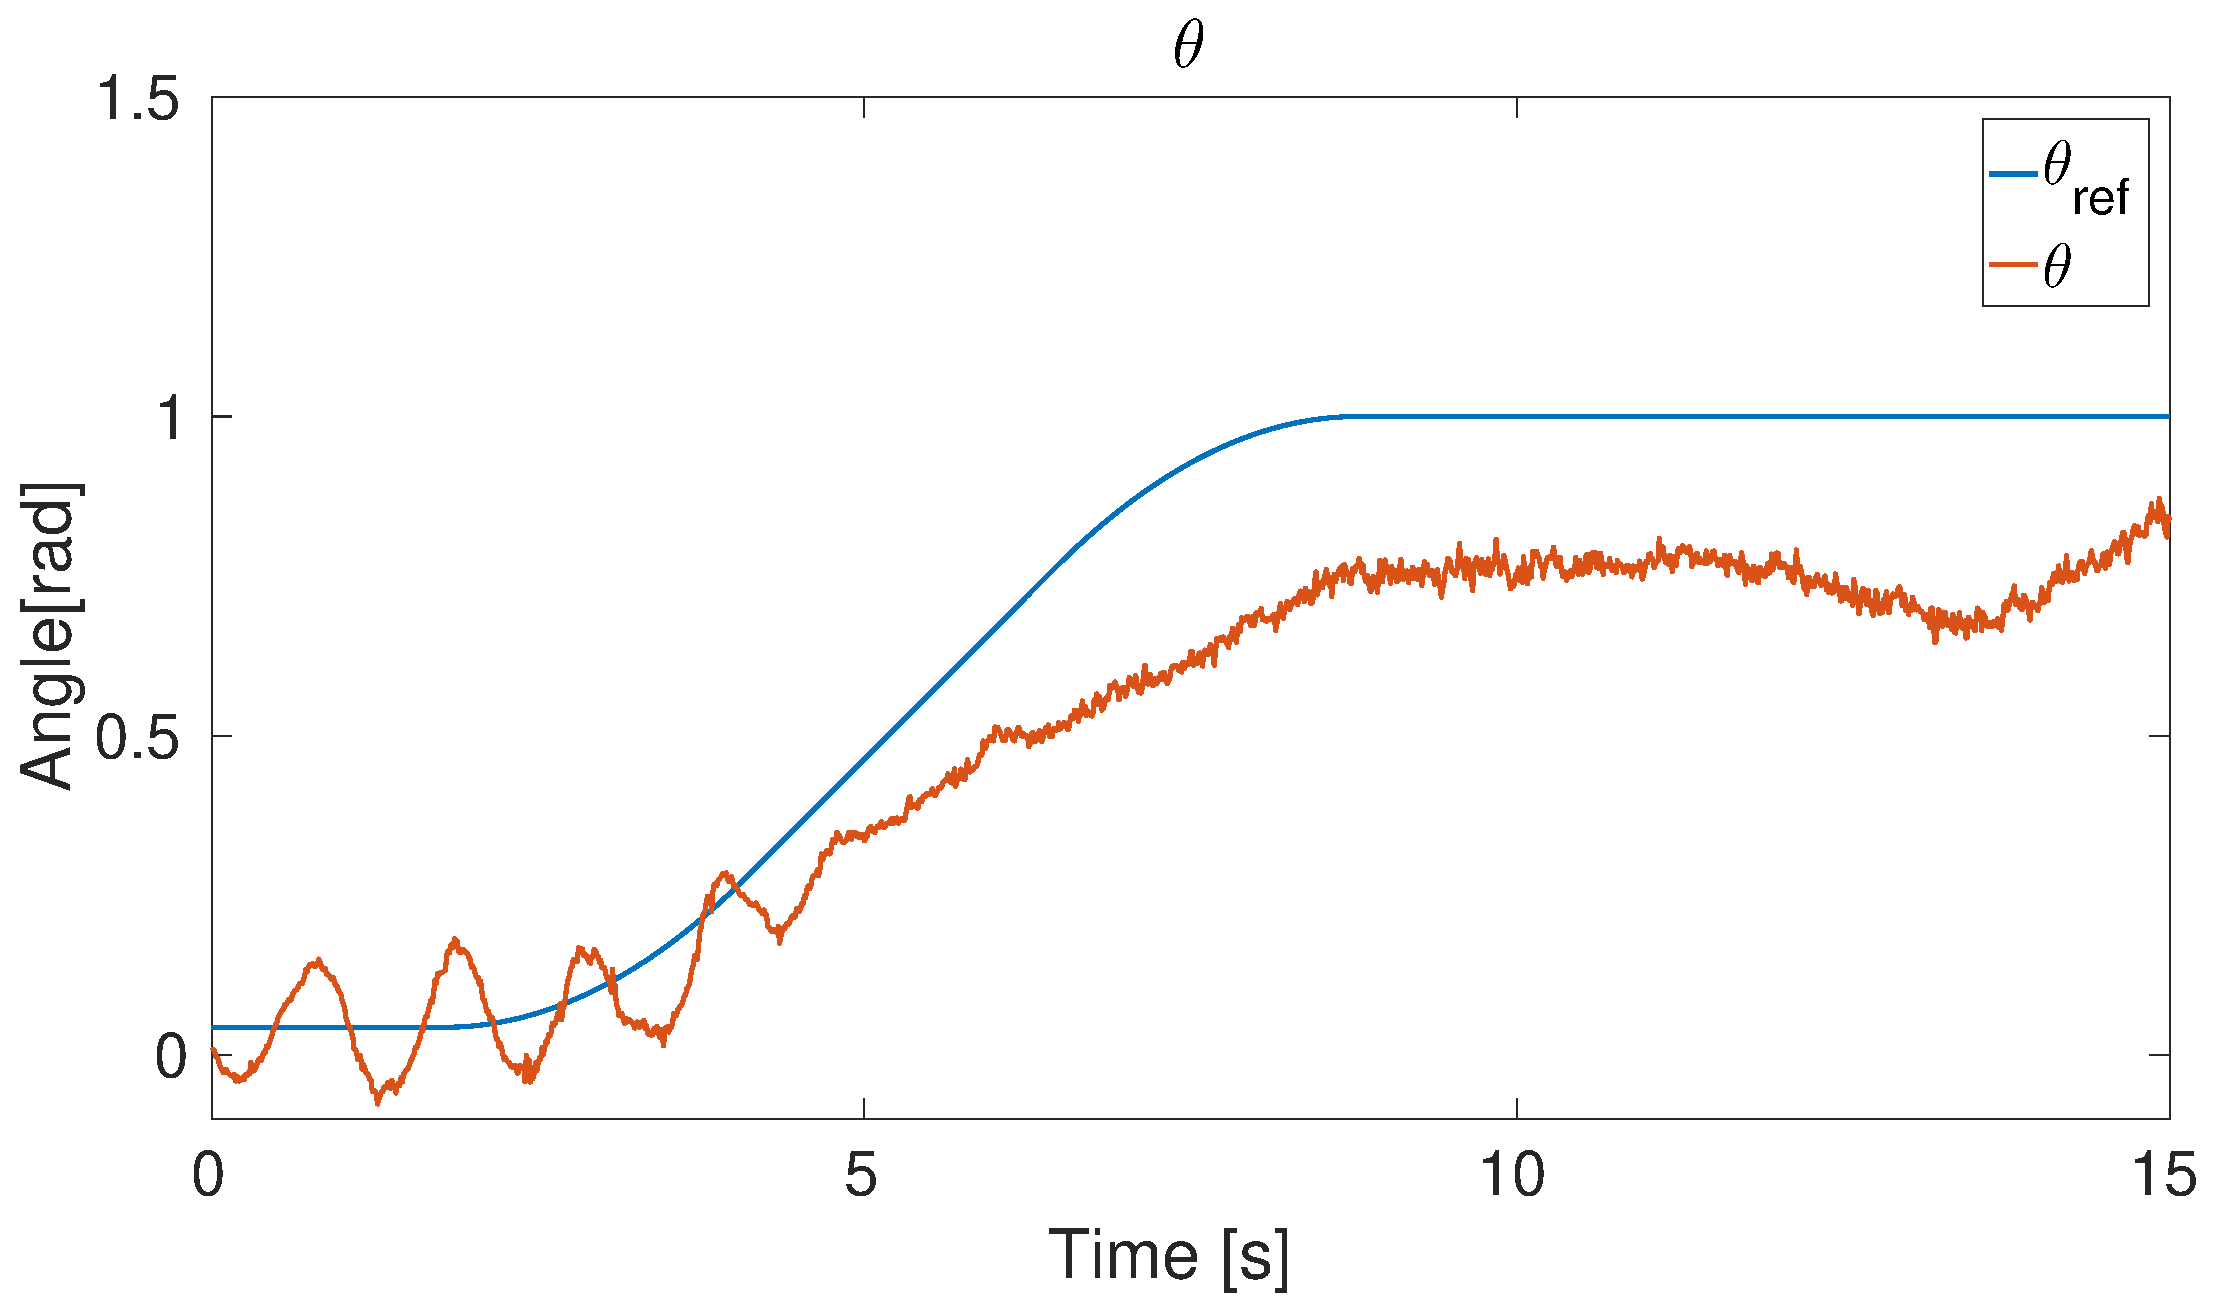
\includegraphics[scale=0.28]{../Master/fig/testStepThetaPhiThetas3e10a1}
}
\end{frame}




%%%%%%%%%Conclusion%%%%%%%%%%%%%%%%%%%%%%%%%%%%%%%%%%%%%%%%%%%%%%%%%%%%%%%%%%%%%%%%%%
\section{Conclusion}
\begin{frame}

\end{frame}
%%%%%%%%%%%%

\end{document}
